%----------------------------------------------------------------------------------------
%	CHƯƠNG 2: CƠ SỞ LÝ THUYẾT
%----------------------------------------------------------------------------------------

\chapter{CƠ SỞ LÝ THUYẾT}
\label{Chapter2}

% =================================================================
%   MỤC 2.1
% =================================================================
\section{Tìm kiếm đối kháng}
% Tiểu mục 2.1.1
\subsection{Lý thuyết trò chơi}

Trong lĩnh vực Trí tuệ nhân tạo, khi đối mặt với các môi trường đa tác tử, lý thuyết trò chơi cung cấp các góc nhìn hệ thống để mô hình hóa hành vi của đối thủ nhằm tìm ra quyết định tối ưu. Có ít nhất ba góc nhìn chiến lược mà hệ thống có thể lấy làm điểm xuất phát để phân tích hành vi:

\begin{itemize}
	\item \textbf{Góc nhìn kinh tế tổng hợp:} Góc nhìn này tiếp cận môi trường dưới dạng một nền kinh tế, cực kỳ phù hợp khi có một số lượng rất lớn các tác tử tham gia vĩ mô. Nó cho phép chúng ta dự đoán các xu hướng tổng hợp (ví dụ: nhu cầu tăng sẽ đẩy giá cả lên cao) mà không cần phải dự đoán chính xác hành động riêng lẻ của từng tác tử cụ thể. Hướng tiếp cận này được áp dụng rộng rãi trong các bài toán tối ưu nguồn lực phức tạp nhưng không phù hợp cho dạng đối kháng tay đôi.
	\item \textbf{Góc nhìn môi trường biến động ngẫu nhiên:} Góc nhìn này xem các tác tử đối kháng đơn thuần là một phần của môi trường động và biến nó thành một môi trường không xác định. Việc mô hình hóa đối thủ theo cách này tương tự như cách xử lý hiện tượng tự nhiên ngẫu nhiên (ví dụ: trời đôi khi mưa và đôi khi không). Cách tiếp cận này dẫu đơn giản nhưng lại bỏ sót một thực tế quan trọng: \textbf{đối thủ đang chủ động tìm mọi cách để đánh bại chúng ta}, trong khi các hiện tượng tự nhiên như mưa hoàn toàn không có ý định hay chiến lược cốt lõi đó.
	\item \textbf{Góc nhìn tìm kiếm cây trò chơi đối kháng:} Chúng ta tiến hành mô hình hóa một cách tường minh hành vi của đối thủ thông qua các kỹ thuật duyệt cây trò chơi nhằm tìm ra chiến lược phản đòn hợp lý nhất
\end{itemize}
Từ góc nhìn tìm kiếm đối kháng này, hệ thống sẽ đi qua một lớp trò chơi có điều kiện hạn chế như cờ Caro để định nghĩa thế nào là một nước đi tối ưu và áp dụng thuật toán \textbf{Tìm kiếm Minimax} làm nền tảng xử lý gốc. Giải thuật này giả định cả hai người chơi đều có lý trí và đưa ra các nước đi hoàn hảo để đối đầu nhau 
%-----------------------------------
%	TIỂU MỤC 2
%-----------------------------------

\subsection{Mô hình hóa cờ Caro bằng Cây trò chơi}

Trò chơi cờ caro được định nghĩa bao gồm các thành phần cốt lõi sau:
\begin{itemize}
	\item \textbf{$S_0$ (Root Node):} Là nút gốc cao nhất của cây trò chơi, biểu diễn trạng thái bàn cờ hoàn toàn trống rỗng khi ván đấu bắt đầu.
	
	\item \textbf{\texttt{TO-MOVE}(s):} Xác định danh tính người chơi có quyền thực hiện nước đi tại trạng thái hiện tại $s$. Trong mô hình đối kháng tay đôi này, quyền quyết định sẽ luân phiên tuần tự giữa hai tác tử: người chơi tối đa hóa lợi ích (MAX) và người chơi tối thiểu hóa lợi ích (MIN). 
	
	\item \textbf{\texttt{Actions}(s):} Trả về danh sách tất cả các nước đi hợp lệ mà một người chơi được phép thực hiện tại trạng thái $s$. Đối với cờ Caro, hành động này là việc đặt một quân cờ vào các vị trí ô lưới còn trống trên bàn cờ. Trong các cài đặt thực tế nhằm tối ưu hiệu năng duyệt cây, tập hợp hành động này thường được giới hạn thu hẹp trong phạm vi các ô trống xung quanh vùng đang có quân cờ để tránh duyệt các ô biệt lập vô nghĩa.
	
	\item \textbf{\texttt{Result}(s, a):} Mô hình chuyển dịch trạng thái, trả về một nút con mới trên cây sau khi hành động $a$ được thực thi thành công tại nút cha $s$. Do môi trường mang tính xác định cao, một cặp $(s, a)$ cố định luôn luôn dẫn đến một kết quả \texttt{Result}(s, a) duy nhất.
	
	\item \textbf{\texttt{IS-TERMINAL}(s):} Hàm logic thực hiện nhiệm vụ quét trạng thái bàn cờ để xác định ván cờ đã đạt đến điều kiện dừng hay chưa. Trận đấu sẽ dừng lại khi xuất hiện một chuỗi chiến thắng gồm đúng 5 quân cờ liên tiếp hợp lệ hoặc khi bàn cờ đã bị lấp đầy hoàn toàn dẫn đến cục diện hòa. Các nút thỏa mãn điều kiện dừng này được gọi là nút lá (Terminal Nodes) và không phát triển thêm nhánh con.
	
	\item \textbf{\texttt{Utility}(s, p):} Hàm lợi ích (còn được gọi là hàm mục tiêu hoặc hàm trả thưởng), xác định giá trị số cuối cùng cho người chơi $p$ khi trò chơi kết thúc ở trạng thái kết thúc $s$.
\end{itemize}

\begin{center}
	\nopagebreak
	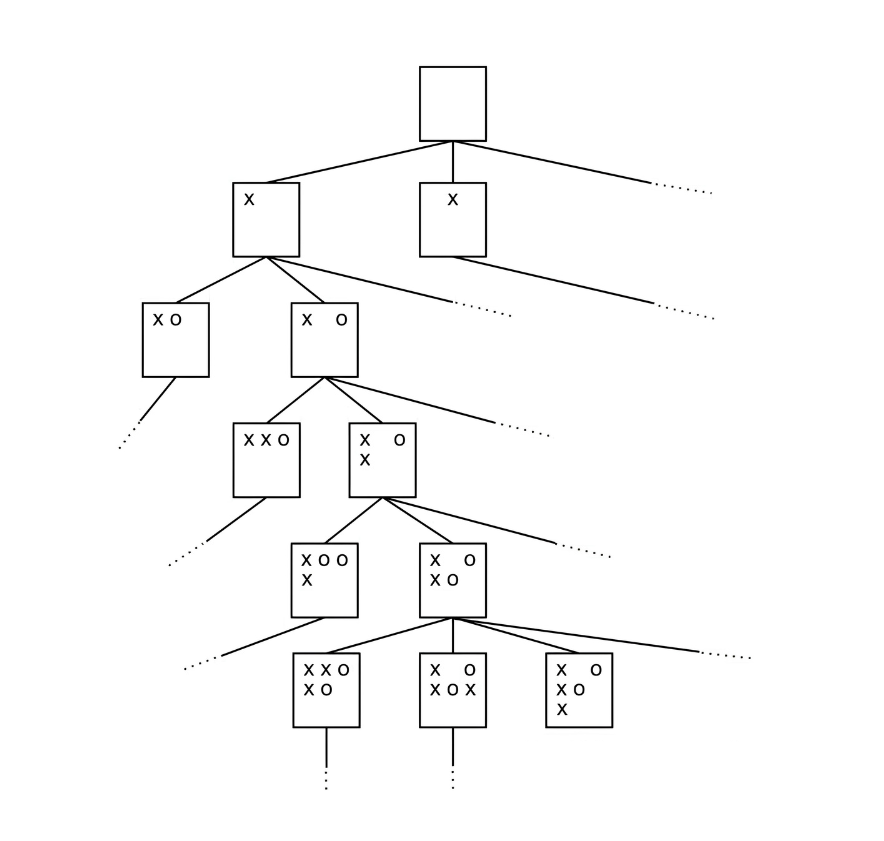
\includegraphics[width=0.55\textwidth]{Figures/Gallery/gametree.png}
	\captionof{figure}{Cây trò chơi của cờ Caro 3x3 (Tic-Tac-Toe)}
	\label{fig:game_tree}
\end{center}
\vspace{0.3cm}

Một tham số kỹ thuật cực kỳ quan trọng chi phối trực tiếp đến cấu trúc hình học và độ phình của cây trò chơi là hệ số phân nhánh $b$, đại diện cho số lượng nước đi hợp lệ trung bình tại mỗi tầng của cây. Đối với bàn cờ Caro tiêu chuẩn kích thước 15x15, ở nước cờ đầu tiên hệ số phân nhánh tối đa lên tới \textit{225} và giảm dần sau mỗi nước đi tiếp theo.
%----------------------------------------------------------------------------------------
%	MỤC 2
%----------------------------------------------------------------------------------------

\section{Thuật toán tìm kiếm Minimax}

Thuật toán Minimax là giải thuật nền tảng được thiết kế chuyên biệt để giải quyết các bài toán tìm kiếm đối kháng trong mô hình trò chơi có tổng bằng không (zero-sum games). Bản chất của đặc tính ``tổng bằng không'' quy định rằng bất kỳ một nước đi nào mang lại lợi thế cho một người chơi sẽ tương ứng mang lại một lượng thiệt hại hoặc hình phạt có giá trị tuyệt đối bằng chừng đó cho người chơi đối phương, nghĩa là cục diện ván cờ luôn được duy trì dưới dạng một cán cân toán học cân bằng và không tồn tại bất kỳ kết quả đôi bên cùng có lợi (win-win outcome) nào. Để vận hành mô hình này, giải thuật phân định hai thực thể tham gia luân phiên bằng tên gọi toán học là MAX (đại diện cho tác tử AI) và MIN (đại diện cho người chơi đối phương), trong đó hai người chơi sẽ thay phiên nhau đặt các quân cờ cho đến khi trận đấu đạt trạng thái kết thúc. Tại các nút lá kết thúc này, các giá trị số học cao sẽ đại diện cho phần thưởng tốt đối với góc nhìn chiến lược của tác tử MAX và đồng thời là kết quả tồi tệ nhất đối với góc nhìn của tác tử MIN.

Về bản chất vận hành, thuật toán Minimax là một chiến lược chơi game mạnh mẽ hoạt động trực tiếp trên cấu trúc cây trò chơi. Cơ chế cốt lõi của giải thuật là việc hình dung ra kịch bản xấu nhất có thể xảy ra từ bất kỳ nước đi nào của bản thân dưới sự phản công thông minh từ phía đối thủ, và sau đó chọn lựa nước đi dẫn đến kịch bản xấu nhất tốt nhất - tức là tìm kiếm giải pháp ``ít tệ nhất'' trong số các tình huống nguy hiểm có thể xảy ra. 

Thuật toán Minimax lựa chọn hành động tối ưu theo tiến trình các bước cụ thể sau:
\begin{enumerate}
	\item \textbf{Khởi tạo cây tìm kiếm giới hạn:} Xây dựng một cây trò chơi biểu diễn toàn bộ các trạng thái có thể mở rộng của trò chơi từ thời điểm hiện tại.
	\item \textbf{Xác định giá trị tại các nút lá giới hạn:} Xác định từng nút lá đại diện cho trạng thái cuối cùng (hoặc trạng thái dừng tại độ sâu giới hạn) và gán cho nó giá trị Minimax tùy thuộc vào việc nó tương ứng với kết quả thắng ($+1$), thua ($-1$) hoặc hòa ($0$) đối với tác tử.
	\item \textbf{Lan truyền ngược giá trị lên các nút cha:} Liên tục truyền các giá trị định lượng đó ngược lên cây để xác định giá trị cho các nút cha. Tiến trình này giả định bạn luôn cố gắng giành chiến thắng (tối đa hóa giá trị lợi ích) và đối thủ của bạn có lý trí sẽ luôn cố gắng khiến bạn thua (tối thiểu hóa giá trị lợi ích của bạn):
	\begin{itemize}
		
		\item \textbf{Nếu nút cha tương ứng với lượt đi của bạn (MAX):} Giá trị Minimax của nút cha sẽ bằng giá trị lớn nhất ($\max$) trong số các giá trị của các nút con trực tiếp, bởi vì bạn luôn muốn tối đa hóa lợi thế và điểm số của bản thân.
		
		\item \textbf{Nếu nút cha tương ứng với lượt đi của đối thủ (MIN):} Giá trị Minimax của nút cha sẽ bằng giá trị nhỏ nhất ($\min$) trong số các giá trị của các nút con trực tiếp, bởi vì hệ thống mặc định đối thủ có lý trí sẽ luôn muốn tối thiểu hóa điểm số để kìm hãm bạn.
	\end{itemize}
	\item \textbf{Ra quyết định nước đi tối ưu:} Tại nút gốc (trạng thái hiện tại của bàn cờ), tác tử AI sẽ luôn luôn lựa chọn hành động dẫn dắt trò chơi dịch chuyển sang nút con có giá trị Minimax cao nhất. Trong trường hợp xuất hiện nhiều nút con có giá trị tối ưu bằng nhau, hệ thống có thể phá vỡ thế cân bằng bằng cách lựa chọn ngẫu nhiên một trong các nước đi đó.
\end{enumerate}

 Mô hình toán học tổng quát chi phối toàn bộ tiến trình 4 bước nêu trên được thiết lập theo công thức đệ quy luân phiên sau:

 $$\text{MINIMAX}(s) = 
 \begin{cases} 
 	\text{UTILITY}(s, \text{MAX}) & \text{if } \text{IS-TERMINAL}(s) \\ 
 	\max_{a \in \text{Actions}(s)} \text{MINIMAX}(\text{RESULT}(s, a)) & \text{if } \text{TO-MOVE}(s) = \text{MAX} \\ 
 	\min_{a \in \text{Actions}(s)} \text{MINIMAX}(\text{RESULT}(s, a)) & \text{if } \text{TO-MOVE}(s) = \text{MIN} 
 \end{cases}$$
 \begin{center}
 	\nopagebreak
 	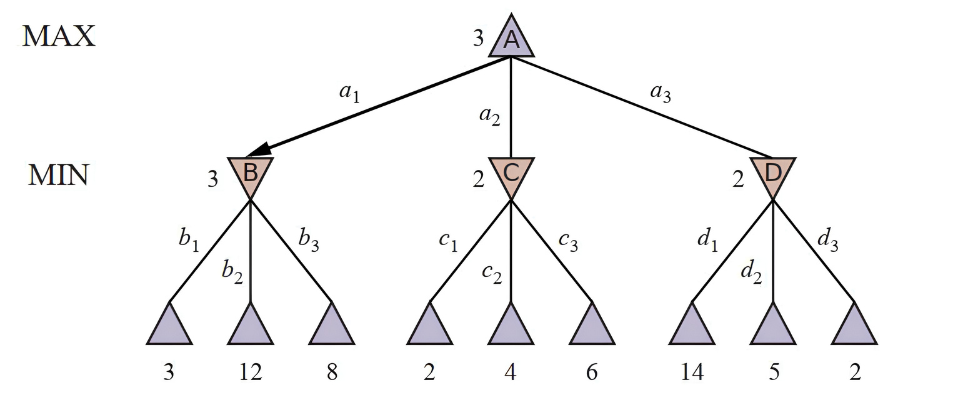
\includegraphics[width=\textwidth]{Figures/Gallery/minimax.png}
 	\captionof{figure}{Sơ đồ cây tìm kiếm đối kháng và tiến trình lan truyền ngược Minimax giữa hai tác tử MAX và MIN}
 	\label{fig:minimax}
 \end{center}
 \vspace{0.3cm}
 Mặc dù giải thuật đảm bảo tìm ra chiến lược tối ưu tuyệt đối, việc phải duyệt toàn bộ cây trò chơi đến tận các nút lá khiến tổng số lượng trạng thái cần tính toán tăng trưởng theo hàm mũ $b^d$. Do đó, độ phức tạp thời gian của thuật toán Minimax trong kịch bản xấu nhất là $\mathcal{O}(b^d)$, trong khi độ phức tạp không gian bộ nhớ lưu trữ các nút trên đường đi hiện tại là $\mathcal{O}(bd)$. 
 
 Đối với các trò chơi sở hữu không gian trạng thái rộng lớn như cờ Caro, sự bùng nổ tổ hợp này đặt ra thách thức cực kỳ lớn cho năng lực tính toán của phần cứng. 
 
 \begin{table}[!htbp]
 	\centering
 	\caption{Minh họa sự bùng nổ tổ hợp số nút cần duyệt theo độ sâu}
 	\label{tab:combinatorial_explosion}
 	\begin{tabular}{|c|c|c|r|}
 		\hline
 		\textbf{Bàn cờ} & \textbf{\textit{b}} & \textbf{\textit{d}} & \textbf{Số nút} \\ \hline
 		\multirow{3}{*}{10x10} & 100 & 1 & 100 \\ \cline{2-4} 
 		& 100 & 2 & 10.000 \\ \cline{2-4} 
 		& 100 & 3 & 1.000.000 \\ \hline
 		\multirow{3}{*}{12x12} & 144 & 1 & 144 \\ \cline{2-4} 
 		& 144 & 2 & 20.736 \\ \cline{2-4} 
 		& 144 & 3 & 2.985.984 \\ \hline
 		\multirow{3}{*}{15x15} & 225 & 1 & 225 \\ \cline{2-4} 
 		& 225 & 2 & 50.625 \\ \cline{2-4} 
 		& 225 & 3 & 11.390.625 \\ \hline
 	\end{tabular}
 \end{table}
 
Sự gia tăng nhanh chóng của số lượng trạng thái như dữ liệu thống kê trên chính là giới hạn vật lý kìm hãm chiều sâu tư duy của AI. Đây cũng là tiền đề cốt lõi thúc đẩy việc nghiên cứu và áp dụng các kỹ thuật cải tiến, tối ưu hóa thọc sâu trực tiếp vào cấu trúc cây trò chơi ở các mục tiếp theo nhằm cắt tỉa bớt các nhánh thừa vô nghĩa mà vẫn bảo toàn tính chính xác của quyết định.
 
\section{Thuật toán cắt tỉa $\alpha$ - $\beta$} 
Nhược điểm lớn nhất của thuật toán Minimax thuần túy là hiện tượng bùng nổ tổ hợp do phải duyệt qua toàn bộ các trạng thái trên cây trò chơi với độ phức tạp thời gian theo hàm mũ $\mathcal{O}(b^d)$, khiến việc tính toán trở nên bất khả thi đối với các trò chơi có hệ số phân nhánh lớn như cờ Caro. Để tối ưu hóa hiệu năng tính toán mà không làm thay đổi kết quả lựa chọn nước đi cuối cùng tại nút gốc, kỹ thuật \textbf{Cắt tỉa Alpha-Beta (Alpha-Beta Pruning)} được tích hợp trực tiếp vào tiến trình duyệt cây theo chiều sâu (DFS). Vì bản chất của Minimax là tìm kiếm theo chiều sâu, tại bất kỳ thời điểm nào, hệ thống chỉ cần xem xét các nút dọc theo một đường dẫn duy nhất trên cây trò chơi. 

Bản chất của kỹ thuật cắt tỉa này là bỏ qua việc đánh giá các nhánh của cây trò chơi mà hệ thống chứng minh được rằng chúng chắc chắn sẽ không ảnh hưởng đến quyết định của các tác tử có lý trí ở nút gốc. Phép cắt tỉa vận hành bằng cách duy trì hai tham số toán học xuyên suốt quá trình tìm kiếm: 
\begin{itemize}
	\item \textbf{Tham số $\alpha$ (Alpha):} Đại diện cho giá trị của sự lựa chọn tốt nhất (giá trị cao nhất) mà hệ thống đã tìm được cho đến thời điểm hiện tại tại bất kỳ điểm lựa chọn nào dọc theo đường đi của tác tử MAX. Về mặt toán học, $\alpha$ đóng vai trò là một ngưỡng chặn dưới (định nghĩa theo tư duy: ``ít nhất là'' - \textit{at least}).
	\item \textbf{Tham số $\beta$ (Beta):} Đại diện cho giá trị của sự lựa chọn tốt nhất (giá trị thấp nhất) mà hệ thống đã tìm được cho đến thời điểm hiện tại tại bất kỳ điểm lựa chọn nào dọc theo đường đi của tác tử MIN. Về mặt toán học, $\beta$ đóng vai trò là một ngưỡng chặn trên (định nghĩa theo tư duy: ``nhiều nhất là'' - \textit{at most}).
\end{itemize}

Thuật toán cắt tỉa Alpha-Beta thực hiện cập nhật liên tục hai tham số này thông qua một tiến trình xử lý liên tục: các giá trị $\alpha$ và $\beta$ hiện thời từ nút cha sẽ được truyền trực tiếp xuống cho các nút con tính toán khi đi sâu xuống cây trò chơi. Tại các nút thuộc lượt đi của MAX, hệ thống nhận các giá trị trả về từ các nút con và liên tục cập nhật tham số $\alpha$ bằng cách lấy giá trị lớn nhất ($\max$) giữa $\alpha$ hiện tại và giá trị của nút con vừa duyệt. Ngược lại, tại các nút thuộc lượt đi của MIN, hệ thống liên tục cập nhật tham số $\beta$ bằng cách lấy giá trị nhỏ nhất ($\min$) giữa $\beta$ hiện tại và giá trị của nút con vừa duyệt.

Tại bất kỳ thời điểm nào trong quá trình duyệt, nếu hệ thống phát hiện ra điều kiện toán học:
$$\alpha \ge \beta$$
Tiến trình cắt tỉa sẽ lập tức được kích hoạt để ngừng duyệt tất cả các nhánh con còn lại của nút hiện tại vì việc duyệt thêm trở nên hoàn toàn vô nghĩa. Phép cắt tỉa này được phân chia thành hai trường hợp cụ thể:

\begin{enumerate}
	\item \textbf{Cắt tỉa xảy ra tại một nút thuộc lượt của MIN (Alpha-cut):} 
	\begin{itemize}
		\item \textbf{Cơ chế:} Khi tác tử MIN tìm thấy một nước đi có giá trị nhỏ hơn hoặc bằng giá trị $\alpha$ hiện thời (ngưỡng chặn dưới mà MAX đã đảm bảo đạt được ở các nhánh trước).
		\item \textbf{Hệ quả:} Do tác tử MIN có lý trí chắc chắn sẽ ưu tiên chọn nước đi thấp hơn hoặc bằng này, nó sẽ khiến giá trị của toàn bộ nút MIN hiện tại không thể vượt qua $\alpha$. Kết quả là nút cha MAX ở tầng trên sẽ không bao giờ lựa chọn nhánh này nữa. Vì vậy, hệ thống lập tức dừng duyệt toàn bộ các nhánh con còn lại của nút MIN hiện tại.
	\end{itemize}
	
	\item \textbf{Cắt tỉa xảy ra tại một nút thuộc lượt của MAX (Beta-cut):} 
	\begin{itemize}
		\item \textbf{Cơ chế:} Khi tác tử MAX tìm thấy một nước đi có giá trị lớn hơn hoặc bằng giá trị $\beta$ hiện thời (ngưỡng chặn trên mà MIN giới hạn cho phép ở tầng trước).
		\item\textbf{Hệ quả:} Do tác tử MAX chắc chắn sẽ chọn nước đi cao hơn hoặc bằng này, nó làm cho giá trị của nút MAX hiện tại chắc chắn vượt qua ngưỡng $\beta$. Điều này dẫn đến việc nút cha MIN ở tầng trên sẽ loại bỏ ngay lập tức việc lựa chọn nhánh này. Vì vậy, tiến trình duyệt các nhánh con còn lại của nút MAX hiện hành lập tức bị bẻ gãy.
	\end{itemize}
\end{enumerate}
 \begin{center}
	\nopagebreak
	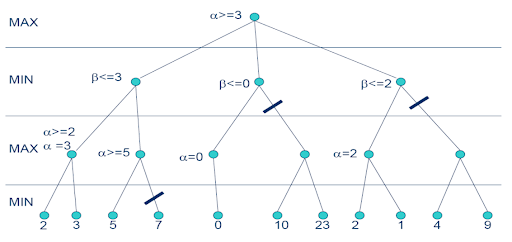
\includegraphics[width=0.8\textwidth]{Figures/Gallery/ab_prun.png}
	\captionof{figure}{Sơ đồ cây tìm kiếm MiniMax có kết hợp cắt tỉa $\alpha$ - $\beta$}
	\label{fig:ab_prun}
\end{center}
Hiệu quả về mặt toán học của phép cắt tỉa Alpha-Beta phụ thuộc hoàn toàn vào thứ tự duyệt các nước đi trên cây trò chơi. Trong trường hợp lý tưởng nhất - khi các nước đi tốt nhất luôn được hệ thống ưu tiên duyệt và đánh giá trước - độ phức tạp thời gian của thuật toán được giảm thiểu một cách đáng kể từ $\mathcal{O}(b^d)$ của Minimax thuần túy xuống chỉ còn:
$$\mathcal{O}\left(b^{\frac{d}{2}}\right)$$

Nói một cách khác, với một thứ tự chọn nước đi hoàn hảo, thuật toán Alpha-Beta có thể giải quyết được một cây trò chơi có độ sâu gấp đôi ($2d$) so với thuật toán Minimax thuần túy trong cùng một quỹ thời gian tính toán. Ngược lại, nếu thứ tự duyệt các nước đi diễn ra hoàn toàn ngẫu nhiên, tổng số nút cần phải kiểm tra đối với một hệ số phân nhánh trung bình sẽ rơi vào khoảng $\mathcal{O}\left(b^{\frac{3d}{4}}\right)$.

Xét về độ phức tạp không gian, do cả hai giải thuật Minimax và Alpha-Beta về bản chất đều vận hành dựa trên nguyên lý duyệt cây theo chiều sâu (DFS), cấu trúc bộ nhớ chỉ đòi hỏi lưu trữ các nút dọc theo một đường đi duy nhất từ nút gốc đến nút lá hiện hành, cùng với các nút anh em chưa được duyệt trực tiếp của chúng. Do đó, độ phức tạp không gian bộ nhớ của thuật toán cắt tỉa vẫn duy trì ổn định ở mức tuyến tính:
$$\mathcal{O}(bd)$$

\section{Giới hạn độ sâu và Hàm đánh giá tĩnh}

Chúng ta không thể xây dựng một cây trò chơi hoàn chỉnh cho trò chơi cờ Caro thay vào đó ta có thể làm như sau:

\begin{itemize}
	\item Giới hạn độ sâu tìm kiếm (tức là xây dựng một cây trò chơi rút gọn đến một độ sâu tối đa nào đó)
	\item Đưa ra một hàm đánh giá heuristic nào đó để đánh giá mức độ tốt hay xấu của mỗi trạng thái nút lá của cây trò chơi đã bị giới hạn độ sâu. 
\end{itemize}

\subsection{Giới hạn độ sâu}

Mặc dù kỹ thuật cắt tỉa $\alpha$ - $\beta$ đã tối ưu hóa mạnh mẽ tiến trình duyệt cây, nhưng đối với những trò chơi có không gian trạng thái khổng lồ như cờ Caro, việc duyệt sâu cho đến khi đạt được trạng thái kết thúc ở tận cuối ván cờ là điều bất khả thi về mặt tài nguyên máy tính. Ở những nước đi đầu tiên, hệ số phân nhánh b có thể lên tới 225, khiến cây trò chơi phình to theo hàm mũ.
Để giải quyết vấn đề bùng nổ tổ hợp này, thuật toán tìm kiếm bắt buộc phải áp dụng kỹ thuật Giới hạn độ sâu. Hệ thống sẽ thiết lập một cơ chế chủ động ngắt tiến trình duyệt cây khi độ sâu tìm kiếm đạt đến một ngưỡng d được định trước (ví dụ trong đồ án này là d=3 hoặc d=4). Tuy nhiên, sự can thiệp này làm nảy sinh một thách thức toán học mới: tại điểm ngắt d, hầu hết các trạng thái bàn cờ đều đang ở cục diện tranh chấp, chưa thực sự kết thúc. Tại các "nút lá tạm thời" này, hệ thống không thể sử dụng hàm Lợi ích đích Utility($s$) để trả về điểm số Thắng/Thua/Hòa tuyệt đối. Nhu cầu cấp thiết lúc này là phải có một cơ chế ước lượng xem cục diện hiện tại đang nghiêng về bên nào, từ đó làm cơ sở để thuật toán Minimax tiếp tục chọn lọc nước đi. 

\subsection{Hàm đánh giá}

Để giải quyết thách thức do việc giới hạn độ sâu để lại, thuật toán sử dụng một Hàm đánh giá (Heuristic Evaluation Function), thường được ký hiệu là $EVAL(s)$, để chấm điểm và ước lượng mức độ lợi thế của cục diện bàn cờ tại trạng thái đó.

Về mặt toán học, hàm $EVAL(s)$ được định nghĩa dưới dạng một hàm tổng tuyến tính có trọng số:
\begin{equation}
	EVAL(s) = w_1 f_1(s) + w_2 f_2(s) + \dots + w_n f_n(s)
\end{equation}

\begin{itemize}
	\item \textbf{$b_i(s)$ (Tần suất xuất hiện):} Đại diện cho số lượng các thế cờ tấn công/phòng thủ cốt lõi (ví dụ: chuỗi 3 quân thoáng hai đầu, chuỗi 4 quân bị chặn) đang tồn tại trên bàn cờ tại trạng thái $s$.
	
	\item \textbf{$w_i$ (Điểm số Heuristic):} Tương ứng với các giá trị điểm số được khai báo tĩnh. Tham số này định lượng mức độ nguy hiểm của từng thế cờ cụ thể (ví dụ: thế 3 thoáng được đánh giá mức độ rủi ro là 670 điểm, trong khi thế 2 thoáng chỉ có 16 điểm).
\end{itemize}

Quá trình tính toán tổng điểm $EVAL(s)$ được hệ thống thực hiện thông qua 3 bước xử lý mảng:
\begin{itemize}
	\item \textbf{Bóc tách tuyến tính:} Hệ thống tiến hành phân rã ma trận bàn cờ $2D$ thành các mảng $1D$ độc lập bao gồm toàn bộ các hàng ngang, cột dọc và các đường chéo. Để tối ưu hóa hiệu năng, thuật toán sẽ chủ động loại bỏ các đường chéo có độ dài nhỏ hơn $4$ ô nhằm tiết kiệm tài nguyên xử lý của CPU, do các cấu trúc ngắn này không đủ không gian hình học để hình thành chuỗi $5$ quân cờ chiến thắng.
	\item \textbf{Quét cửa sổ trượt:} Sử dụng các khung bộ lọc có kích thước linh hoạt (tương ứng từ $4, 5,$ đến $6$ ô cờ) trượt dọc theo từng mảng $1D$ đã bóc tách. Quá trình này giúp hệ thống nhận diện, phân loại mẫu hình và đếm chính xác số lượng tần suất xuất hiện $f_i(s)$ của từng thế cờ chiến thuật đang hiện diện trên bàn cờ.
	\item \textbf{Tính tổng trọng số:} Tiến hành tổng hợp và nhân tích chập ma trận giữa tần suất xuất hiện $f_i(s)$ vừa quét được với bộ điểm số trọng số hằng số $w_i$ được quy định sẵn trong từ điển để trả về giá trị điểm số cuối cùng của hàm tổng $Eval(s)$, làm căn cứ quyết định cho các tầng đệ quy kế tiếp.
\end{itemize}


\section{Hồi quy Logistic}
Hồi quy Logistic là một thuật toán học máy phân lớp thống kê được sử dụng để dự đoán xác suất của một đầu ra nhị phân ($0$ hoặc $1$). Trong bài toán lượng giá trạng thái trò chơi đối kháng, thuật toán này đóng vai trò thiết lập mối quan hệ giữa các đặc trưng cấu trúc trên bàn cờ và khả năng dẫn đến chiến thắng.

Bản chất của Hồi quy Logistic là việc lấy một hàm tổng tuyến tính của các biến đầu vào (đặc trưng thế cờ) và đưa qua một hàm phi tuyến tính gọi là \textbf{hàm Sigmoid} (hoặc hàm Logistic) để ánh xạ kết quả về khoảng giá trị xác suất $(0, 1)$.

Công thức toán học của hàm số Sigmoid có dạng như sau:
\begin{equation}
	\sigma(z) = \frac{1}{1 + e^{-z}}
\end{equation}

Trong đó, biến $z$ đại diện cho một hàm tổ hợp tuyến tính của các đặc trưng đầu vào $x_i$ kết hợp với bộ trọng số hệ số hồi quy $w_i$ tương ứng:
\begin{equation}
	z = w_0 + w_1 x_1 + w_2 x_2 + \dots + w_n x_n
\end{equation}
	
Khi áp dụng vào bài toán, giá trị đầu ra của $\sigma(z)$ đại diện cho xác suất chiến thắng của một trạng thái cục diện bàn cờ hiện hành. Quá trình huấn luyện mô hình thực chất là việc tối ưu hóa hàm mất mát Binary Cross -  Entropy để tìm ra bộ tham số trọng số $w_i$ tối ưu nhất, làm cơ sở khoa học vững chắc cho việc định lượng điểm số Heuristic thay vì thiết lập thủ công.
